\documentclass[a4paper]{article}
\usepackage[utf8]{inputenc}
\usepackage[russian]{babel}
\usepackage[margin=1in]{geometry}
\usepackage{float}
\usepackage{graphicx}
\usepackage{setspace}
\usepackage{indentfirst}
\usepackage{subfiles}
\usepackage{textcomp}
\usepackage{xcolor,listings}

\lstset{upquote=true}
\title{Курсовая работа по Базам Данных}
\author{Шулайкин Д.А.}
\begin{document}
\onehalfspacing
\thispagestyle{empty}

\begin{center}
Министерство образования и науки Российской Федерации
\vspace{10pt}

Федеральное государственное бюджетное образовательное учереждение высшего образования "Ивановский государственный энергетический университет имени В.И. Ленина"
\vspace{40pt}

Кафедра ПОКС
\vspace{40pt}

{ \LARGE \textbf{Отчет по курсовой работе} } \\
Дисциплина: ``Базы данных'' \\
Тема: ``Проектирование базы данных информационной системы для аквапарка'' \\
\end{center}

\vspace{330pt}

\begin{flushright}
\textbf{Выполнил:} \\
ст. гр. 2-42в \\
Шулайкин Д.А. \\

\textbf{Проверила:} \\
д.т.н., профессор Ратманова И.Д.
\end{flushright}

\vspace{40pt}

\begin{center}
	Иваново 2019
\end{center}

\pagebreak
\begin{center}
	\LARGE
	\textbf{Реферат}
\end{center}
	Пояснительная записка 24 стр., 3 рис., 23 табл. \\ \\
	АКВАПАРК, ЗОНА ОТДЫХА, БАЗА ДАННЫХ, SQL, ПРОЕКТИРОВАНИЕ \\ \\ 
	Объектом исследования является аквапарк. \\ \\ 
	Цель работы: спроектировать и разработать базу данных средствами Microsoft. \\ \\ 
	В качестве СУБД используется docker образ microsoft-mssql-server. \\ \\
	Во введение обосновывается задание и цель работы. \\ \\
	Первый раздел посвящен анализу предметной области. \\ \\ 
	Второй раздел посвящен проектированию базы данных. \\ \\
	Третий раздел посвящен запросам. \\ \\
	Четвертый раздел посвящен бизнес-логике приложения. \\ \\
	В заключении подводится результат проделанной работы.

\pagebreak
\tableofcontents
\pagebreak

\section{Введение}
\subsection{Задание}
Аквапарк предлагает своим клиентам отдых и развлечения в трех зонах: аквапарк, сауны, кафетерий.
Зоны различаются стоимостью одной минуты пребывания в них(для кафетерия - 0 руб.) и стоимостью дневного абонемента.
Клиенты расплачиваются посредством магнитных браслетов. 
Каждый браслет хранит количество минут, проведенных клиентом в каждой зоне, сумму, 
потраченную в кафетерии и величину залога, внесенного при входе.
На выходе все траты пересчитываются и посетителю возвращают разницу или берут с него доплату.
\subsection{Цель работы}
Выполнить курсовую работу на тему «проектирование и разработка базы
данных средствами Microsoft»

\section{Анализ предметной области}
\subsection{Описание таблиц}

\subsubsection{Посещения}
После посещения сервиса для посетителя создается запись, которая содержит длительность посещения и ссылки на посетителя и сервис.

\subsubsection{Посетители}
\emph{handle} - никнейм, который посетитель может поменять в любое время. 
Такой идентификатор удобно использовать в пользовательском интерфейсе.

\subsubsection{Абонементы}
При наличии абонемента в зону отдыха, за время нахождения в ней для посетителя не списываются средства, хотя запись о пребывании все равно создается.
Действуют от момента покупки до конца текущего дня.

\subsubsection{Сервис или зона отдыха}
Сервис характеризуется названием, ценой в минуту(\emph{normalprice}) и ценой абонемента в копейках(\emph{seasonpass}).

\subsubsection{Чеки}
Заказ человека в кафе, характеризуется , содержит в себе заказанные блюда и их количества, и временем.
% Возможно добавить статус заказа (Например: готовится, ожидает, завершен и т.д)

\subsubsection{Запись меню}
Одно блюдо из заказа и его количество.

\subsubsection{Меню}
Меню содержит названия и цены доступных блюд в кафе.
% Возмножно добавить поля категории из списка категорий блюд(напитки или еда и т.д.) и доступность для заказа.

\subsubsection{Платежи}
Переводы средств с счета на другой счет. Возможны следующие варианты:

\begin{enumerate}
\item \emph{from} = NULL, \emph{to} != NULL - Средства вводятся в систему
\item \emph{from} != NULL, \emph{to} != NULL - Средства перемещаются от одного пользователя к другому
\item \emph{from} != NULL, \emph{to} = NULL - Средства выводятся из системы
\end{enumerate}

\subsection{Концептуальная модель}
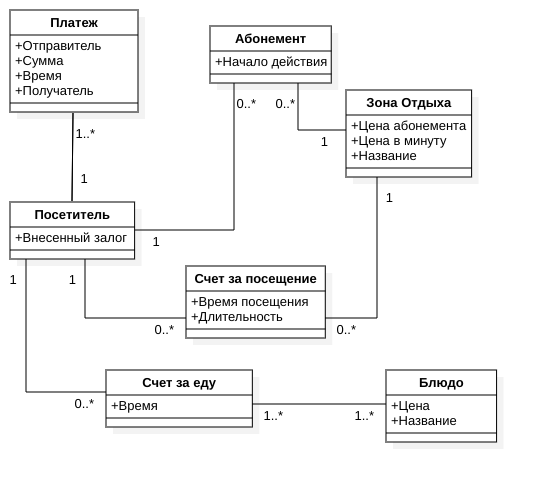
\includegraphics[width=5in]{img/concept.png}
\subsection{Логическая модель}
\includegraphics[width=5in]{img/logic.pdf}

\section{Создание базы данных}
\subsection{Сервисы}
\subfile{subfiles/1.1_create_services}
\subfile{subfiles/2.1_show_services}

\subsection{Посетители}
\subfile{subfiles/1.2_create_customers}
\subfile{subfiles/2.2_show_customers}

\subsection{Абонементы}
\subfile{subfiles/1.3_create_passes}
\subfile{subfiles/2.3_show_passes}

\subsection{Посещения}
\subfile{subfiles/1.4_create_bills}
\subfile{subfiles/2.4_show_bills}

\subsection{Меню}
\subfile{subfiles/1.5_create_cafeitems}
\subfile{subfiles/2.5_show_cafeitems}

\subsection{Чеки}
\subfile{subfiles/1.6_create_cafeorders}
\subfile{subfiles/2.6_show_cafeorders}

\subsection{Запись меню}
\subfile{subfiles/1.7_create_orderItems}
\subfile{subfiles/2.7_show_orderitems}

\subsection{Платежи}
\subfile{subfiles/1.8_create_deposits}
\subfile{subfiles/2.8_show_deposits}

\subsection{Физическая модель}
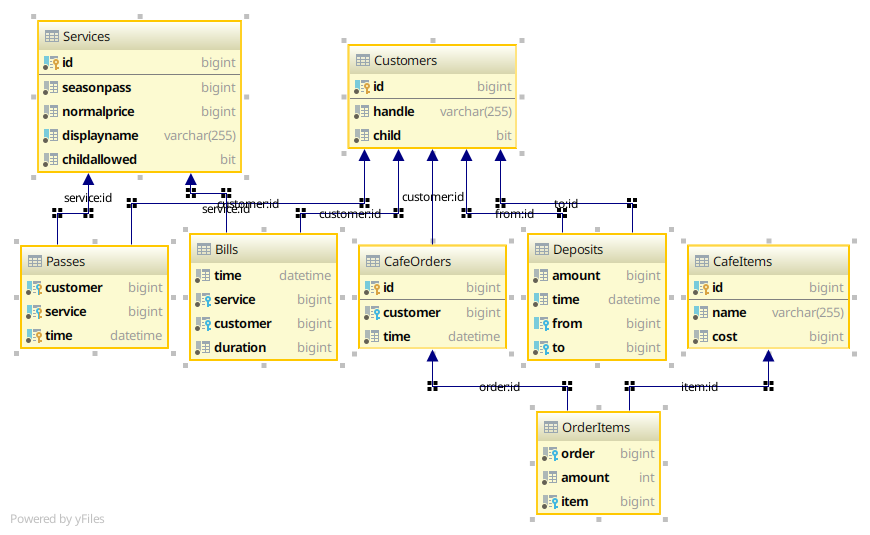
\includegraphics[width=5in]{img/db.png}

\section{Запросы}

% Задание:
% 7-10 запросов:
% - объединение таблиц
% -с условием WHERE
% -с группировкой
% -с условием HAVING
% -с агрегатными функциями
% -подзапросы : с EXISTS и объединение UNION
% -оператор выбора CASE

\subsection{Вывести все предметы меню начинающиеся на букву ``m''}
\subfile{subfiles/3.1_getcafeitems}

\subsection{Вывести все входящие платежи для какого-либо посетителя}
\subfile{subfiles/3.2_getcustdeposits}

\subsection{Вывести стоимость посещения сервиса с учетом абонемента}
\subfile{subfiles/3.3_get_bill_cost}

\subsection{Вывести сумму трат посетителя в кафе}
\subfile{subfiles/3.4_get_cafe_expenses}

\subsection{Вывести стоимость заказа}
\subfile{subfiles/3.5_get_order_cost}

\subsection{Вывести сумму трат посетителя на зоны отдыха}
\subfile{subfiles/3.6_get_cust_bills}

\subsection{Вывести сумму трат посетителя на абонементы}
\subfile{subfiles/3.7_get_passes_expenses}

\subsection{Вывести сумму баланс всех посетителей на текущий момент}
\subfile{subfiles/6.8_get_cust_summary}

\subsection{Вывести все траты посетителя в хронологическом порядке}
\subfile{subfiles/3.9_union_query}

%\subsection{Запрос с слиянием таблиц}
%Необходимо получить все услуги которыми пользовался человек с их наименованием
%\subfile{subfiles/get_cust_bills}

%\subsection{Запрос с условием}
%Необходимо получить все переводы на счет какого-либо человека \textit{id}
%\subfile{subfiles/get_cust_deposits}

%\subsection{Запрос с агрегатными функциями}
%Для нахождения стоимости заказа в кафе необходимо взять сумму от всех произведений цены входящих в заказ блюд на количества этих блюд.
%\subfile{subfiles/get_order_cost}

%\subsection{Запрос с подзапросом}

%\subsection{Запрос с оператором выбора}
%Для нахождения стоимости услуги для конкретного человека необходимо рассмотреть несколько случаев, зависящих от наличия абонемента.

%\begin{enumerate}
	%\item Если у человека нет абонемента, то стоимость услуги вычисляется как произведения поминутной стоимости на количество забилленых минут.
	%\item Если у человека есть абонемент, то услуга предоставляется бесплатно.
	%\item Если человек купил абонемент во время предоставления услуги, то стоимость вычисляется как произведение стоимости на минуты, но учитываются только время до покупки абонемента
%\end{enumerate}

%\subfile{subfiles/get_bill_cost}

%\subsection{Запрос с группировкой}
%Довольно часто хочется получить остаток со счета у конкретного человека, 
%он на равен разнице суммы депозитов и суммы всех расходов в кафе, на абонементы и на услуги.

%Довайте создадим виртуальную таблицу которая отражает \textit{id} в текущий остаток по счету человека.
%Для этого добавим группировку в запросы нахождения стоимостей.

%Запрос на нахождение всех трат в кафе какого-либо человека  \textit{id}
%\subfile{subfiles/get_cafe_expenses}

%Запрос на нахождение стоимости всех абонементов какого-либо человека  \textit{id}
%\subfile{subfiles/get_passes_expenses}

%\subsection{Запрос с объединением таблиц}

%Запрос позволяет вывести время всех происходящих событий с посетителем и их тип.

%\subfiles{subfiles/union_query}
\section{Логика приложения}
\subsection{Виртуальные таблицы}
\subsubsection{Таблица расходов посетителей на абонементы}
\subfile{subfiles/4.1_create_view_passes}
\subfile{subfiles/5.1_show_view_passes}

\subsubsection{Таблица расходов посетителей на зоны отдыха}
\subfile{subfiles/4.2_create_view_bills}
\subfile{subfiles/5.2_show_view_bills}

\subsubsection{Таблица трат в кафе посетителей}
\subfile{subfiles/4.3_create_view_cafeexpenses}
\subfile{subfiles/5.3_show_view_cafeexpenses}

\subsubsection{Таблица переводов другим пользователям}
\subfile{subfiles/4.4_create_view_shared_money}
\subfile{subfiles/5.4_show_view_shared_money}

\subsubsection{Таблица поплнений баланса}
\subfile{subfiles/4.5_create_view_deposits}
\subfile{subfiles/5.5_show_view_deposits}

\subsubsection{Сводная таблица по посетителям для рассчета баланса}
\subfile{subfiles/4.6_create_view_balance}
\subfile{subfiles/5.6_show_view_balance}

\subsection{Хранимые процедуры}
\subsubsection{Возвращает сумму входящих платежей посетителя}
\subfile{subfiles/7.1_create_proc_deposits}

\subsubsection{Возвращает сумму потраченную на зоны отдыха посетителем}
\subfile{subfiles/7.2_create_proc_bills}

\subsubsection{Возвращает сумму потраченную в кафе посетителем}
\subfile{subfiles/7.3_create_proc_cafe}

\subsubsection{Возвращает сумму потраченную на абонементы посетителем}
\subfile{subfiles/7.4_create_proc_passes}

\subsubsection{Возвращает сумму переведенную другим посетителям от посетителя}
\subfile{subfiles/7.5_create_proc_shared_money}

\subsubsection{Возвращает все траты посетителя в хронологическом порядке}
\subfile{subfiles/7.6_create_proc_user_history}

\subsubsection{Возвращает все траты посетителя в хронологическом порядке}
\subfile{subfiles/7.7_create_proc_balance}
Вызов процедуры:
\subfile{subfiles/8.1_exec_proc_balance}
Результатом вызова должно быть сообщение ``Balance = 3000''

\subsection{Триггеры}
\subsubsection{Триггер на проверку баланса при заказе еды в кафе}
\subfile{subfiles/9.1_trigger_check_balance}

\section{Заключение}
	В результате проектирования базы данных была построена концептуальная,
логическая и физическая модели предметной области. В среде разработки была реализована
база данных. Были выполнены запросы к базе данных, созданы хранимые процедуры на
выборку данных и триггер после изменения данных на языке SQL.
\end{document}